\documentclass{standalone}

\usepackage[OT1]{fontenc}
\renewcommand*\familydefault{\sfdefault}
\usepackage{helvet,sfmath}
\usepackage{siunitx}

\usepackage{tikz}
\usetikzlibrary{arrows,calc,patterns}
% \usetikzlibrary{intersections, calc, arrows.meta}
\usepackage{tikz,tkz-euclide}

\definecolor{Liquid1}{RGB}{157, 110, 144}
\definecolor{Liquid2}{RGB}{232, 211, 230}
\definecolor{Note}{RGB}{54, 40, 76}
\definecolor{Rotate}{RGB}{107, 46, 61} 


\begin{document}

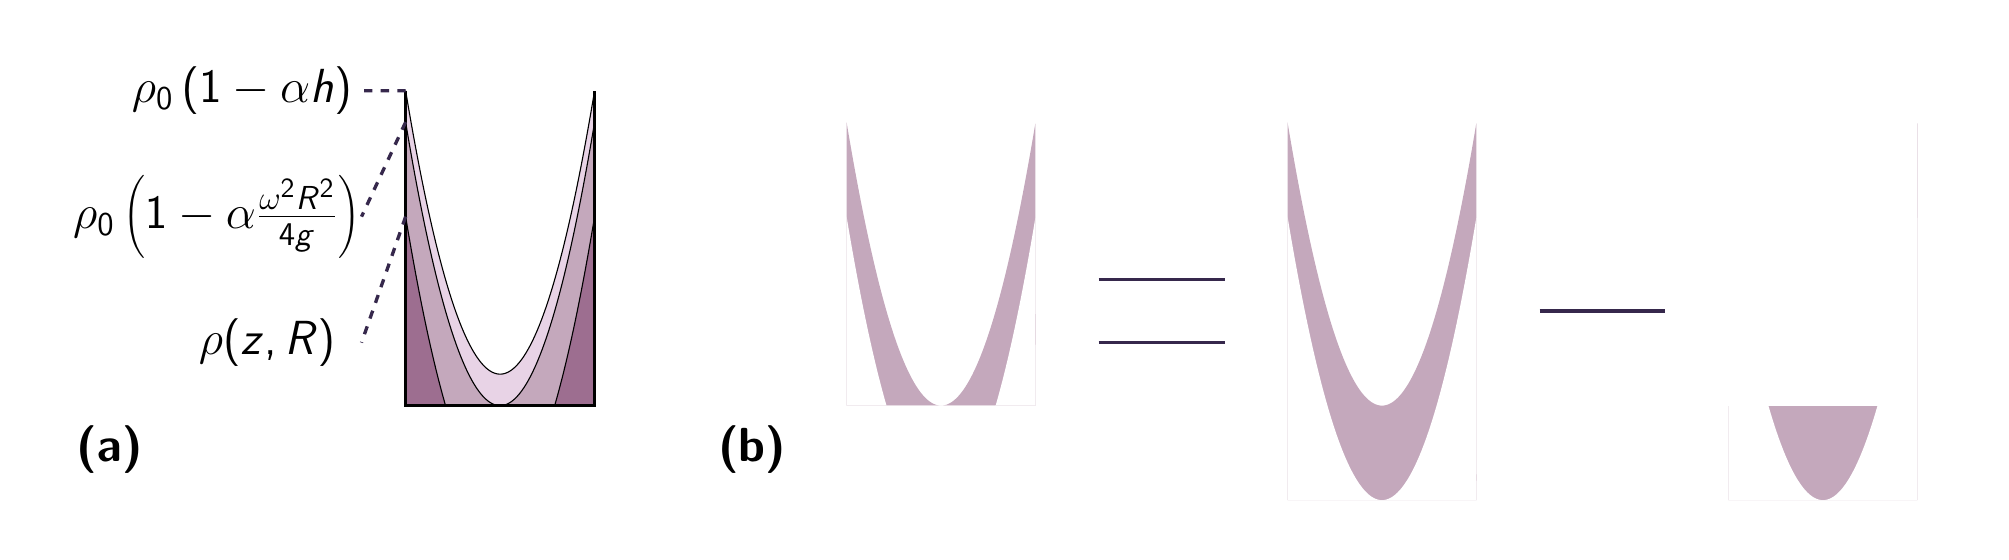
\begin{tikzpicture}[scale=0.8]
    %%Background
    \draw[draw=none] (-5,-1) to (26,7);

    %% Initial state
    \draw[fill = Liquid2, domain=-1.5:1.5, samples = 200, smooth, variable=\t] 
    plot ({2.5+\t}, {1.5+2*\t*\t}) to (4,1) to (1,1);
    \draw[fill = Liquid1!60, domain=-1.5:1.5, samples = 200, smooth, variable=\t] 
    plot ({2.5+\t}, {1+2*\t*\t}) to (4,1) to (1,1);
    \draw[fill = Liquid1, domain=-1.5:1.5, samples = 200, smooth, variable=\t] 
    plot ({2.5+\t}, {-0.5+2*\t*\t}) to (4,1) to (1,1);
    \draw[draw=none, fill=white] (1,1) rectangle (4,-1);
    \draw[very thick] (1,6) to (1,1) to (4,1) to (4,6);

    \draw[dashed, very thick, Note]
    (1,6) to (0.3,6)
    (1,5.5) to (0.3,4)
    (1,4) to (0.3,2)
    ;

    \draw
    (-1.6,6) node{\LARGE\(\rho_0 \left( 1 - \alpha h \right)\)}
    (-2,4) node{\LARGE\(\rho_0 \left( 1 - \alpha \frac{\omega^2 R^2}{4g} \right)\)}
    (-1.2,2) node{\LARGE\(\rho(z,R)\)}
    ;

    %%
    \draw[draw=none, fill = Liquid1!60, domain=-1.5:1.5, samples = 200, smooth, variable=\t] 
    plot ({9.5+\t}, {1+2*\t*\t}) to (11,1) to (8,1);
    \draw[draw=none, fill = white, domain=-1.5:1.5, samples = 200, smooth, variable=\t] 
    plot ({9.5+\t}, {-0.5+2*\t*\t}) to (11,1) to (8,1);

    %%
    \draw[draw=none, fill = Liquid1!60, domain=-1.5:1.5, samples = 200, smooth, variable=\t] 
    plot ({16.5+\t}, {1+2*\t*\t}) to (18,-0.5) to (15,-0.5);
    \draw[draw=none, fill = white, domain=-1.5:1.5, samples = 200, smooth, variable=\t] 
    plot ({16.5+\t}, {-0.5+2*\t*\t}) to (18,-0.5) to (15,-0.5);

    %%
    \draw[draw=none, fill = Liquid1!60, domain=-1.5:1.5, samples = 200, smooth, variable=\t] 
    plot ({23.5+\t}, {1+2*\t*\t}) to (25,-0.5) to (22,-0.5);
    \draw[draw=none, fill = white, domain=-1.5:1.5, samples = 200, smooth, variable=\t] 
    plot ({23.5+\t}, {-0.5+2*\t*\t}) to (25,-0.5) to (22,-0.5);
    \draw[draw=none, fill=white] (22,1) rectangle (25,6);

    %%
    %=
    \draw[very thick, Note]
    (12,2) to (14,2)
    (12,3) to (14,3)
    ;
    %-
    \draw[very thick, Note]
    (19,2.5) to (21,2.5)
    ;

    \draw
    (-3.7,0.3) node{\LARGE \textbf{(a)}}
    (6.5,0.3) node{\LARGE \textbf{(b)}}
    ;
    
\end{tikzpicture}

\end{document}
